% !TeX root = ../main.tex

\chapter{Literature Review}

\section{Related Work on Carpooling}



\subsection{Dial-a-ride Problem}

When it comes to carpooling, the dial-a-ride problem could be one of the best discussions about this kind of scenario. Dial-a-rider problem (DARP) is a problem for finding vehicle routes to serve users with requests with specific origins and destinations, with objective to minimize cost or maximize satisfied demand \cite{cordeau_dial--ride_2007}. DARP has been widely researched for about 50 years \cite{wilson1971scheduling} and is considered as an NP-hard problem \cite{cordeau_branch-and-cut_2006}. There are many variations in the discussion. Cordeau and Laporte \cite{cordeau_dial--ride_2007} indicate that DARP mainly consists of the following factors:

\begin{itemize}
  \item Vehicles: There might be $1$ or $n$ vehicles in the system. Most DARP studies assume that vehicles are with homogeneous capacity; some studies may use a heterogeneous fleet with different capacity.
  \item Requests: A request usually consists of these parts: passengers, origins, destinations, and time constraints. Static or dynamic is also a significant concern. For a static DARP, all the ride requests will be known in advance, and the central scenario is to allocate all the resources once. A dynamic DARP usually discusses ride request planning in a specific time window. For better understanding, we will use ride requests instead of requests.
  \item Routes: Routes of the road network usually consist of length and duration.
  \item Detour: Because a route of DARP is aggregate from many must-pass nodes proposed by ride requests. Rather than the shortest path, every passenger may have a detour.
\end{itemize}

A DARP is a kind of problem that consists of $n$ must-pass nodes with the lowest cost. We will use a Steiner tree problem for finding routes.

\subsection{Steiner Tree Problem}

A Steiner tree problem is to find a minimum cost tree in given subset vertices of a given graph. When it comes to the Steiner tree, a minimum spanning tree problem can be mentioned together. While a minimum spanning tree problem is to find a minimum total weight that the links have to go through all the vertices in a given graph, a Steiner tree problem treats the vertices as terminal and non-terminal vertices. All terminals must go through, and the non-terminal vertices are allowed to contain to reduce cost \cite{wu_steiner_nodate}. Figure 2.1 as an example; this figure is an undirected graph $G=(V, E, w)$ with nonnegative weights. A set of vertices $L \subset V$ is the terminals. The minimal Steiner tree is to find a tree that passes all the terminals that can include other vertices in the graph. We could find a Steiner minimal tree shown in Figure 2.2 with cost = 5. According to Foulds and Graham \cite{foulds_steiner_1982}, finding a Steiner minimal tree (SMT) is an NP-Complete problem, which has no deterministic algorithms to solve in the polynomial time. As a result, we tend to use heuristic approaches to this problem.

\begin{figure}[htp]
  \centering
  \captionsetup{justification=centering}
  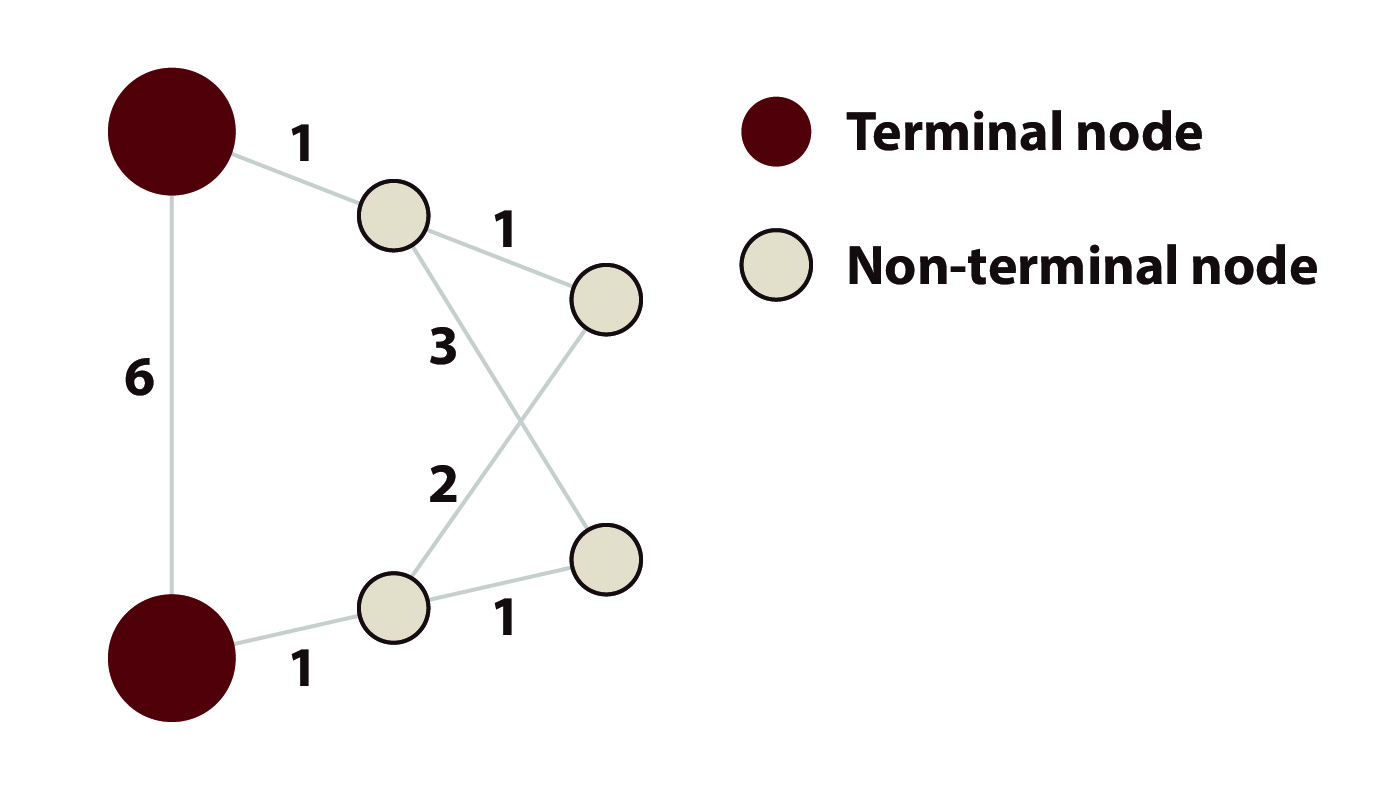
\includegraphics[width=10cm]{figures/steiner_1.jpg}
  \caption{Example graph of a Steiner tree problem}
\end{figure}

\begin{figure}[htp]
  \centering
  \captionsetup{justification=centering}
  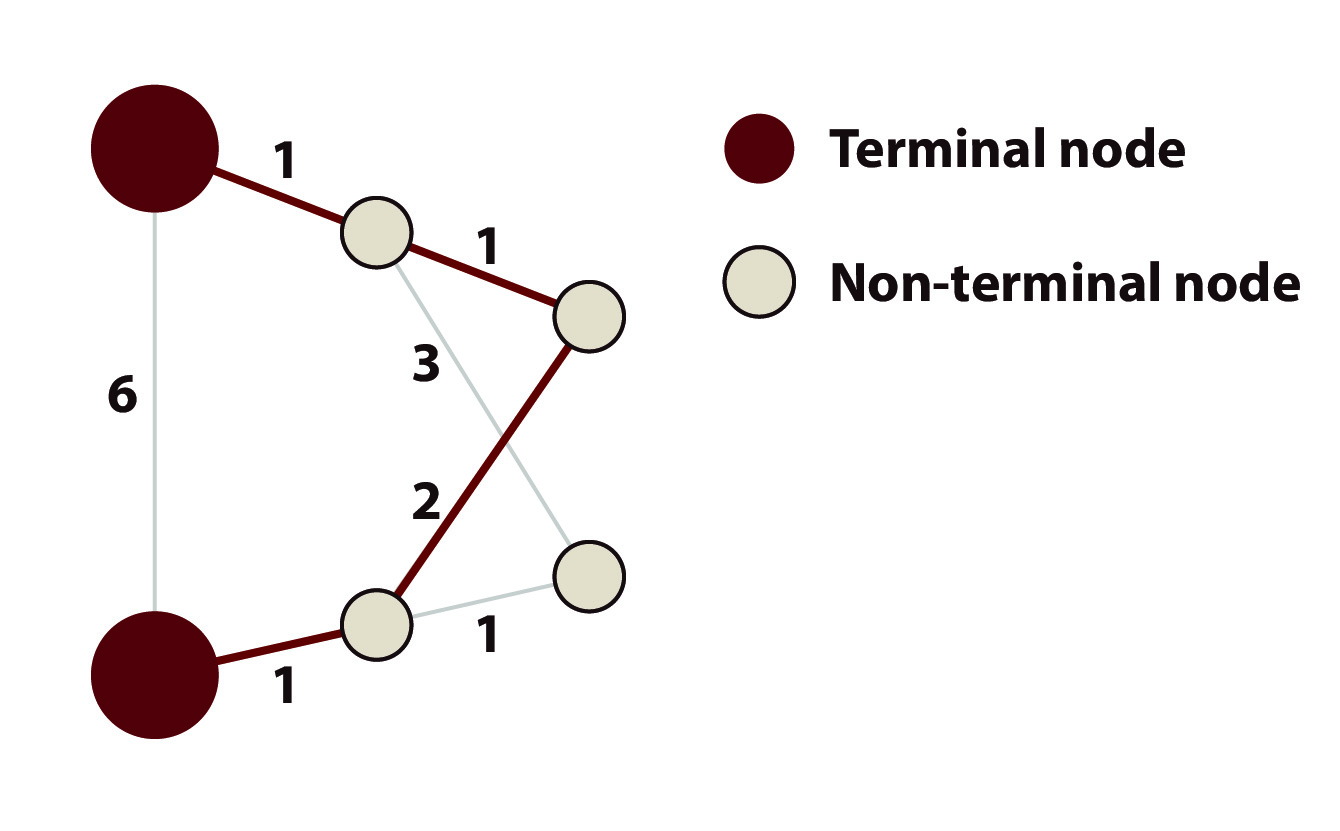
\includegraphics[width=10cm]{figures/steiner_2.jpg}
  \caption{Steiner minimal tree with cost = 5}
\end{figure}

\section{Fairness}

Fairness is the central issue in our research. According to the Cambridge dictionary definition, fairness is "the quality of treating people equally or in a way that is right or reasonable" \cite{noauthor_fairness_nodate}. There are many factors to be considered when it comes to carpooling. One of them is the mechanism of dispatching ride requests to drivers. Suppose a driver in the carpooling system is not treated equally, such as not receiving any ride request in the rush hour while others receive a lot. In that case, the driver might choose not to use the carpooling system. However, getting rid of unequal ride requests dispatching is not easy. There are many possibilities for drivers to think they are treated equally or unequally. For instance, one may think it is equal to receive the same ride requests as others. In contrast, another may think to be treated unequally for participating in carpooling for a long time. To get rid of the issue in such a resource allocation scenario, we define fairness in a mathematical approach to measure fairness. There are many indices to measure the fairness of resource allocation \cite{jain_99-0045_nodate}. In this paper, we use Raj Jain's approach, Jain's fairness index \cite{jain_quantitative_1998}, to know the status of ride request allocation by calculation.

\subsection{Jain's Fairness Index}

Jain's fairness index is a metric to measure the fairness of the resource allocation in a system, which is used in the networking engineering field. By definition, there are $n$ users share resource in a system, a user $i \in \{1,2,3,...,n\}$ allocates $x_i$ resource \cite{jain_quantitative_1998}. The following is the formula:

$Firness\ Index = f_A(x) = \frac{\left(\sum\limits_{i=1}^{n} x_i\right)^2}{n \sum\limits_{i=1}^{n} x_i^2}$

The index ranges from $\frac{1}{n}$ to $1$. When there is only one user monopoly to all resource, which means the others get no resource, the fairness index will be $\frac{1}{n}$. It is the most unfair scenario. When all the users get the same resource, the fairness index will be $1$, which is the fairest scenario.